\subsubsection{Regressione}

Procediamo ora con l'analisi del grafico del dislivello $d$ in funzione della temperatura $\theta$.
In base ai dati da noi raccolti abbiamo ottenuto il seguente risultato, illustrato in figura (\ref{fig:dislivello_temperatura}).

\begin{SCfigure}
    \centering
    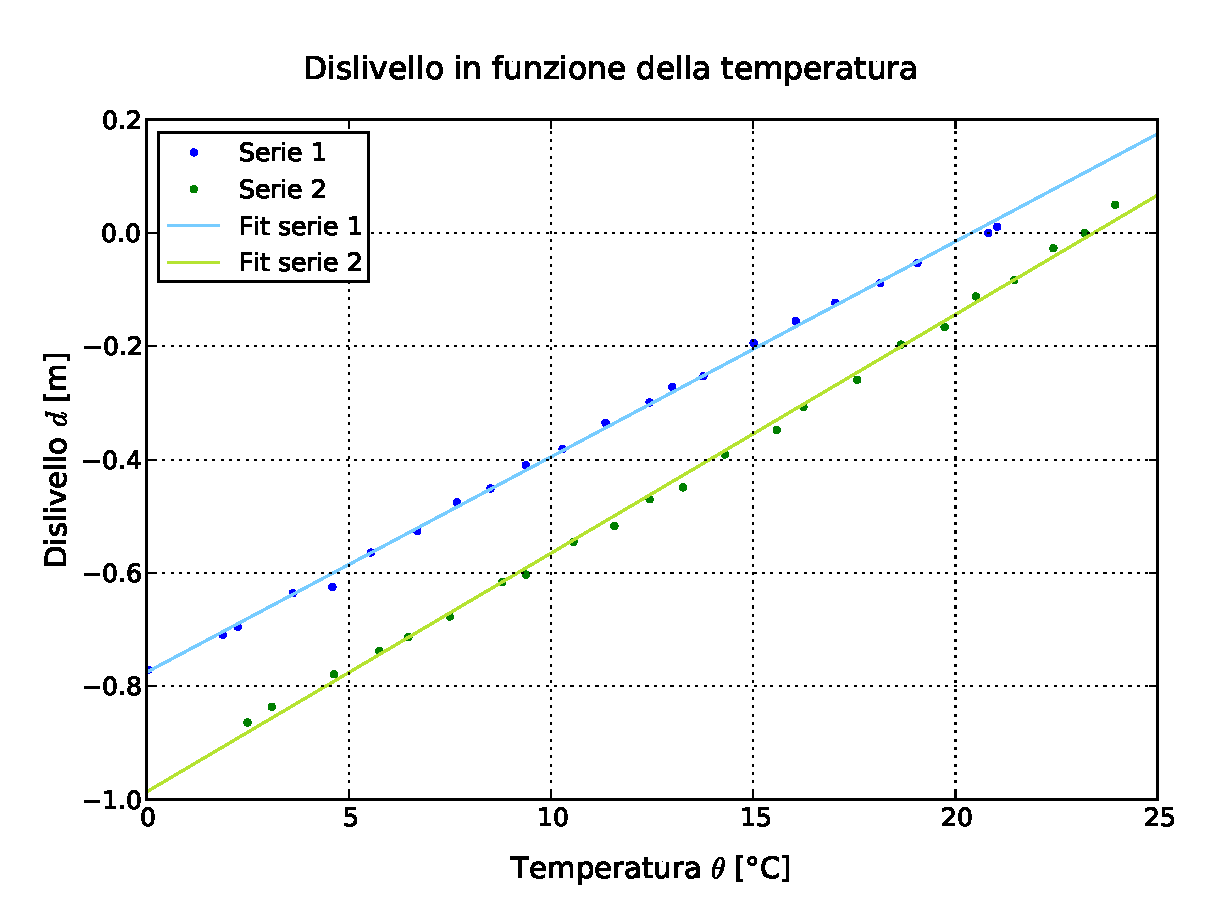
\includegraphics[width=120mm]{immagini/dislivello_temperatura.pdf}
    \caption{Il seguente grafico rappresenta}
    \label{fig:dislivello_temperatura}
\end{SCfigure}
%
Si vede che esiste una correlazione tra la temperatura $\theta$ e dislivello $d$ ed è anche approssimativamente lineare.
Con il metodo dei minimi quadrati, abbiamo quindi trovato la funzione lineare

\begin{equation}
	d \,=\, A + B\,\theta
	\label{h_theta}
\end{equation}
%
che meglio si adatta ai dati da noi raccolti. L'intera procedura qui descritta è stata
applicata ad entrambe le serie di dati separatamente.

Come primo passo abbiamo eseguito dei fit prelimiari sulle due serie di dati,
al fine di trasferire l'incertezza dalla temperatura al dislivello.
Per fare ciò occorre minimizzare la funzione

\begin{equation}
    \sum_{i=1}^{N} \frac{(d - A' - B'\theta)^2}{(\delta d)^2}
    \label{eq:min_quad}
\end{equation}
%
Durante questa fase si è tenuto conto solamente dell'incertezza $\delta d$ sul dislivello. Per calcolare i minimi
di (\ref{eq:min_quad}) si sono usate le formule:

\begin{equation}
    \left(
    \begin{array}{c}
        A' \\
        B'
    \end{array} 
    \right)
    =
    M^{-1}
    \left(
    \begin{array}{c}
        \sum \frac{d}{\delta d} \\[2mm]
        \sum \frac{\theta d}{\delta d}
    \end{array} 
    \right)
    \qquad \qquad
    \text{dove}
    \qquad
    M =
    \large
    \left(
    \begin{array}{c c}
        \sum \frac{1}{\delta d^2} & \sum \frac{\theta}{\delta d^2} \\[2mm]
        \sum \frac{\theta}{\delta d^2} & \sum \frac{\theta^2}{\delta d^2}
    \end{array} 
    \right)
    \label{eq:min_quad}
\end{equation}
%
Una volta calcolato $B'$ si è trasferito l'errore dalla temperatura al dislivello nel seguente modo

\begin{equation}
    \delta d\ped{tot} = \sqrt{\delta d^2 + (B'\delta \theta)^2}
\end{equation}
